\documentclass{subfiles}
\begin{document}
\begin{figure}[!h]
    \centering
    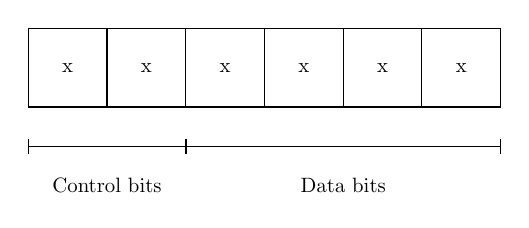
\begin{tikzpicture}[scale = 1, every node/.style={scale = 0.75}]
        \draw (0, 0) rectangle (6, -1);
        \foreach \i in {0, ..., 6}{
                \draw (\i, 0) to (\i, -1);
            }

        \foreach \i in {0.5, ..., 5.5}{
                \draw (\i, -0.5) to (\i, -0.5) node {x};
            }

        \draw[|-|] (0, -1.5) to (2, -1.5);
        \draw[|-|] (2, -1.5) to (6, -1.5);

        \draw (1, -2) -- (1, -2) node {Control bits};
        \draw (4, -2) -- (4, -2) node {Data bits};
    \end{tikzpicture}
    \caption{Codifica dei colori su Commodore Amiga.tex}
    \label{Fig:5.6}
\end{figure}
\end{document}